Different models and languages offer diverse ways to express concepts, such as parallelism or asynchrony.
In this section we evaluate how successful and easy it is to express parallelism using task-based models.  
A good proxy to evaluate how complex a particular implementation is the number of lines of code it takes.
Despite being a metric proposed some decades ago, comparing different programming models in terms of the total number of code lines
is still a valid metric. Indeed, recent publications make an extensive use of it~\cite{Vandierendonck:2011:PPG:2001252.2001265,Dongarra20081}.

%\subsection{Expressiveness}
%\edit{In the Parsec suite we encounter a diverse
%set of parallelization strategies, which however can be grouped into data-parallelism, pipeline parallelism and hybrid between data and pipeline
%parallelism (e.g. \texttt{facesim}).  We were able to express at least the same amount of parallelism in all the 10 benchmarks we used for this study,
%compared to the Pthreads and OpenMP versions.  Additionally, in the cases of \texttt{bodytrack} and \texttt{facesim} we were able to express additional
%parallelism with the use of dataflow annotations and tasks.  Note that in the case of \texttt{dedup}, we adopted a parallelization method with less available
%parallelism than in the case of Pthreads.  We were also able to implement the original Pthreads \texttt{dedup} version but for performance reasons we adopted
%the version with less parallelism.   Section~\ref{sec:implementation} explains this decision in detail.}


%\edit{Although we were able to implement 10 out of the 10 benchmarks, it is possible that we could obtain better results and express additional parallelism in some
%cases, but not with the current standard syntax that OpenMP 4.0 offers.  As discussed in Section \ref{sec:implementation}, the current syntax could benefit from
%extensions that could express data dependencies among irregular and dynamic data structures.  The current OpenMP 4.0 standard is focused on continuous data structures.}

\begin{figure*}[!htbp]
        \centering
        \begin{subfigure}[b]{0.8\textwidth}
                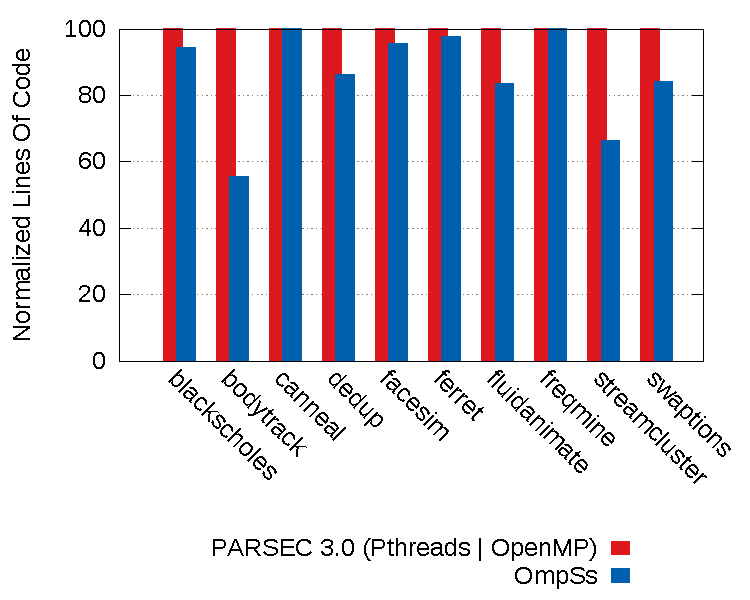
\includegraphics[width=\textwidth]{ifcg/figures/absolute_loc_norm}%
                \caption{Comparison between all source files.}%
                \label{fig:absolute_loc}
                \vspace{0.4cm}
        \end{subfigure}%
				\hfill
        \begin{subfigure}[b]{0.8\textwidth}
        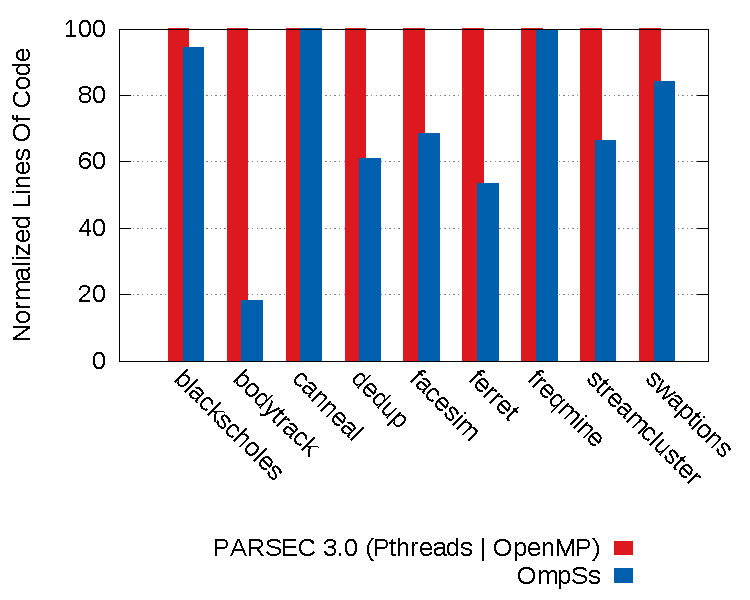
\includegraphics[width=\textwidth]{ifcg/figures/relative_loc_norm}%
        \caption{Comparison between only source files containing parallel code.}%
        \label{fig:relative_loc}%
        \end{subfigure}%
  \caption{Comparison of lines of code between our task-based implementations and the original Pthreads or OpenMP versions.}
        \label{fig:loc_comparison}
\end{figure*}


\subsection{Lines Of Code}
\label{sec:lines}
The reduction of the lines of code (LOC) attests to a more compact and readable code.
%keeping in mind that the actual 
%algorithm complexity remains unchanged.}
In some of our PARSEC task-based implementations, a simple pragma directive replaced application 
specific schedulers, scheduling queues, thread pooling mechanisms and lock synchronization.
We do not change the algorithm in any of the task-based parallel strategy implemented in the PARSEC suite.
Figure~\ref{fig:absolute_loc} shows a normalized comparison between the lines of code of our task-based implementations and the original Pthreads/OpenMP implementations of the PARSEC 3.0 distribution.
The PARSEC 3.0 versions we refer to are always the Pthreads versions, except in the case of \texttt{freqmine} where, since there is no Pthread version available, the OpenMP2.0 version is taken as reference.
We preprocess all source files so that they only contain lines of code relevant to the respective programming model\footnote{PARSEC benchmarks contain mixed serial, Pthreads, OpenMP and TBB source code, and make use of macros to enable conditional compilation for only one programming model at a time.}.
%The LOC column in Table~\ref{tab:parsec} shows the total lines of code for each application, counting all source files.
%Upon careful inspection we can observe that the task-based version requires less lines of code, however parallel code is only a fragment of the sources
%for most applications.  
Figure \ref{fig:relative_loc} shows the total lines of code comparison when we only consider files that are relevant to the parallel 
implementation, that is, files that contain calls to Pthreads or task invocations, asynchronous I/O implementations, atomic primitives, etc.
In this graph we see that the reductions in terms of lines of code of our task-based strategies are significant.
In case of \texttt{bodytrack}, we are able to remove 81\% of the code lines. Since \texttt{Bodytrack} implements its own scheduler to deal with load balancing, there is much room for code reductions by replacing this ad-hoc mechanisms for a few pragma annotations.

By using tasks and dataflow relations, it is very easy to implement pipelines.  We adopt this approach for both \texttt{dedup} and \texttt{ferret}, 
which result in a significant decrease in LOC (38\% and 46\%, respectively). Figure~\ref{lst:ferret-ompss} shows the pipeline code for \texttt{ferret}.  All that is required is
to taskify the different pipeline stages and make sure that dataflow relations force in-order execution of tasks in the same pipeline instance. The Pthreads version requires the implementation
 of queues between each stage, which must also be safe to use by multiple threads and concurrent accesses.
\texttt{Streamcluster} and \texttt{fluidanimate} task-based versions also reduce lines of code by 33\% and 21\% respectively, by removing the need for an additional, user implemented, barrier library. 
\texttt{Blackscholes} and \texttt{swaptions} are relatively simple applications, containing only one do-all parallel loop each.
In these cases the LOC difference is minimal (0.5\% and 15\%, respectively). 
In the cases of \texttt{canneal} and \texttt{freqmine} we see no difference in LOC. 
\texttt{Canneal} is not a data parallel application and in both cases Pthreads and tasks are used merely as thread launching mechanism, while the synchronization effort is essentially the same. 

It is worth noting that conventional synchronization primitives can still be used with tasks, without penalizing the programmer.
\texttt{Freqmine} is implemented in OpenMP, which excels at parallelizing loops with very little effort from the programmer and is the ideal programming model for this application. 
In our implementation we simply taskify the loops, essentially not affecting LOC.
\texttt{Facesim} also benefits from the tasks-based approach by 37\%, as the queues required to schedule work have been 
completely removed. 
Overall, we see that the task-based model reduces code size and by \AVERAGELOC{} on average.

